\documentclass{article}

\usepackage{graphicx}

\title{{\bf An expression signature for p53 status in human in human breast cancer predicts mutation status, transcriptional effects, and patient survival}\\{First part}}
\author{Alexis Grimaldi, Alexandros Pittis, Oriol Vall\`{e}s}

\begin{document}

\maketitle

\begin{abstract}
In this work we extract 20 random samples from GSE3494 dataset, used in paper {\it "An expression signature for p53 status in human breast cancer predicts mutation status, transcriptional effects, and patient survival"}. Our analysis focuses on differentially expressed genes between p53 mutant and wild-type, and here we present the first step of the analysis cycle of microarray data for the IEO project.
\end{abstract}


\section{Introduction}
The p53 tumor suppressor is a critical regulator of tissue homeostasis, and its inactivaction at the gene or protein level confers cellular properties conducive for oncogenesis and cancer progression. Mutations in p53 occur in $>50 \%$ of human cancers and the mutational status of p53 is prognostic in many malignancies. In breast cancer, p53 mutations are associated with worse overall and disease/free survival, independent of other risk factors, and have been implicated in resistance to anticancer therapies.\par
The study we focus on asks itself whether distinctive 32-gene expression patterns exist for p53 mutant and wild-type breast tumors. In order to respond this, the authors proceeded to microarray analysis of a collection of frozen tissues from a cohort found in Uppsala County, Sweden. Transcript profiles of 251 primary breast tumors were determined by using {\it Affymetrix U133} oligonucleotide microarrays, 58 of which had p53 mutations (that resulted in changes in protein expression) and 193 were p53 wild-type.\par
The distinct issues that the study addressed were :
\begin{enumerate}
	\item {\bf P53+ and p53- are molecularily distincts.}
On this point, the paper highlights the fact that most of the top expressed genes are clustering differently in p53 mt and p53 wt tumors.
They also show that p53 status correlates well with ER status (p53 wt with ER positive) and tumor grade (p53 mt with higher tumor grade).
	\item {\bf A gene expression classifier predicts p53 status in independent breast and liver cancer data sets.}
p53 signature genes were chosen thanks to diagonal linear discriminant analysis. Those genes were used to successfully determine, thanks to monte carlo simulations, whether their clustering into different branches could be used to predict p53 status.
	\item {\bf Transcript Analysis of p53 Pathway Genes Corroborates Tumor Clas- sifications.}
Here they show that p53 target genes expression level corroborate with p53 level. This observation is reinforced by functional correlation, yet at a smaller extent.
	\item {\bf The p53 Signature Predicts Outcome Better Than p53 Mutation Status Alone.}
Here is shown that p53 status gives less directly prognostic of patient survival rate than when considering p53 signature genes. More precisely, they show that women with p53 sequence-wt tumors, yet exhibiting the mt-like expression signature, have a greater likelihood of dying from their cancer
	\item {\bf The p53 Signature Predicts Outcome in Independent Therapy-Specific Data Sets.}
The reliability of outcome prediction based on p53 signature genes expression is here assessed in other datasets, in which patients are treated with various methods : doxorubicin, 5FU, mitomycin, tamoxifen, or radiation.
	\item {\bf The p53 Signature Genes Are Not Canonical p53 Targets.}
Functional annotation of the p53 signature genes shows that p53 signature genes are not known p53 target genes, nor do they present p53 binding sites or are implicated in the p53 pathway.
\end{enumerate}
\newpage
\section{Quality Assessment Methodology}
We extracted the data from {\it GSM3494} dataset, placed on {\it http://www.ncbi.nlm.n\\*ih.gov/pubmed/16141321}, which contains a total number of 502 samples. For each one of the 251 patients two distinct microarray analysis were performed by using different platforms HGU1338A and HGU1338B. The following analysis was carried on on a subset of 20 randomly selected samples, half of which were p53 mutant and the other half wild-type as to p53. It was decided to restrict our analysis to only one (A) of the platforms in order to avoid the possible difficulties that could arise from combining them.\par
The phenotypic data associated with the dataset (table, Appendix), corresponding to the clinicopathological variables of the Uppsala cohort, consists of:
\begin{itemize}
	\item ID of the patient
	\item p53 status (mutant or wild-type)
	\item DLDA classifier result
	\item DLDA error
	\item Elston histologic grade Estrogen Receptor (ER) status
	\item PgR status
	\item age at diagnosis
	\item tumor size (mm) 
	\item Lymph node status
	\item DSS TIME (Disease-Specific Survival Time in Years) 
	\item DSS Event (Disease-Specific Survival Event)
\end{itemize}

\subsection{Microarray Data Visualization. Quality Assessment}
We proceed to the Quality Assessment using the {\it Bioconductor} package of R. Once using R, we created an {\it Affybatch} object using the following samples ({\it GSM: 79306, 79165, 79253, 79340, 79287, 79191, 79202, 79211, 79325, 79342, 79232, 79354, 79322, 79153, 79151, 79296, 79249, 79323, 79139 and 79293}), with customized metadata based on the headers of the given phenotypic data. Afterwards, in order to check for the presence of poor quality samples, we produced $MA$ plots, $NUSE$ plots and $RLE$ plots, from which we obtained satisfactory results, as all samples seemed to satisfy the quality standards: 
\begin{enumerate}
	\item $MA$ plots (fig. ~\ref{fig:maplot}) have to be its points around the $0$ value and not much spread out (that is, with low values for the median and $IQR$). As our data fits this criterion, we conclude there are no significant intensity-dependent biases in our microarray analysis.
	\item plotting the {\it Normalized Unscaled Standard Errors} ($NUSE$; fig. ~\ref{fig:nuseplot}) does not give any sample significantly elevated or spread out when compared with the other samples.
	\item all samples are around the $0$ value and not significantly spread out in the {\it Relative Log Expression} ($RLE$; fig. ~\ref{fig:rleplot}) plot, so that we may conclude no samples have poor quality and no filtering is actually needed.
\end{enumerate}

\begin{figure}[ht]
\centerline{\fbox{\includegraphics[width=1\textwidth]{A_MAplot.png}}}
\caption{$MA$ plot for raw data of $A$ batch}
\label{fig:maplot}
\end{figure}

\begin{figure}[h]
\centerline{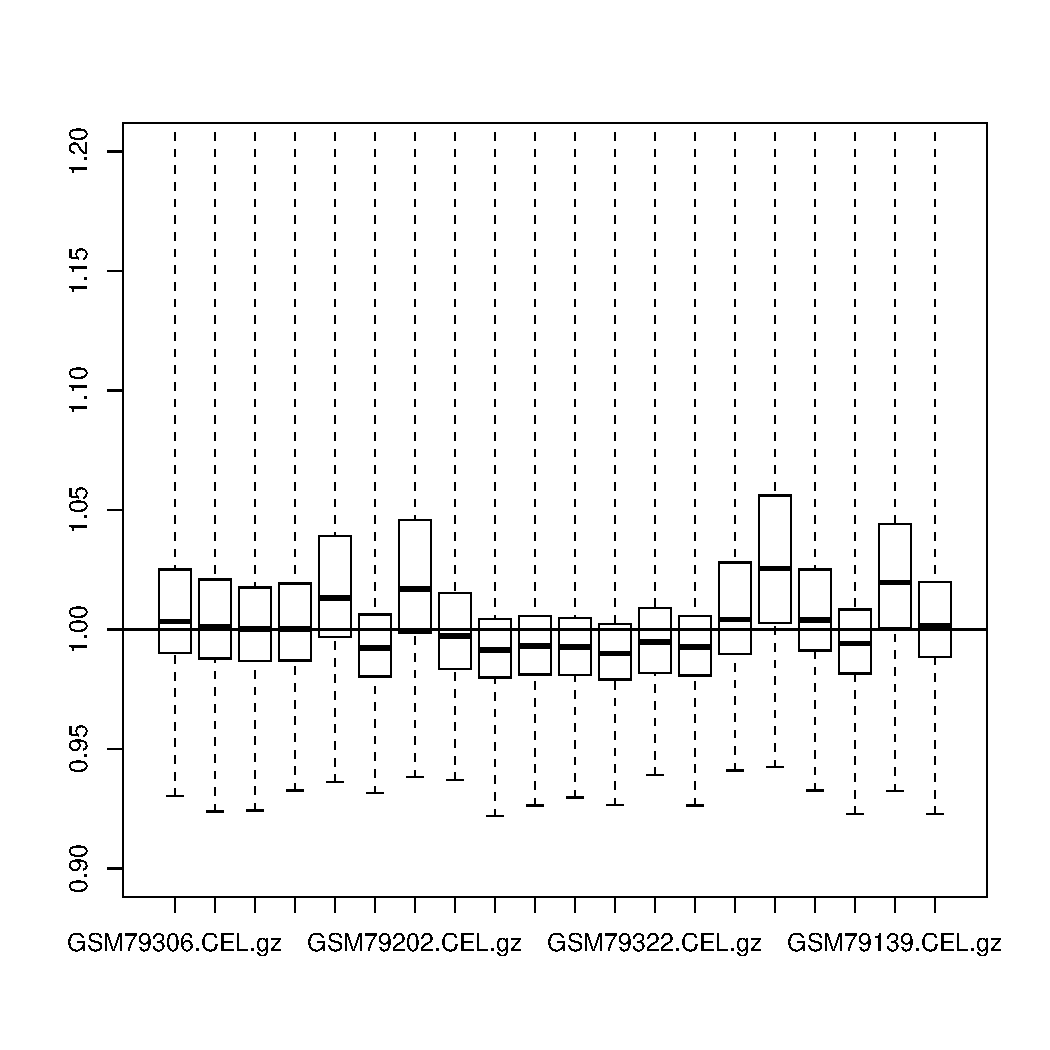
\includegraphics[width=0.45\textwidth]{A_NUSEplot.pdf}}
\caption{$NUSE$ plot for raw data of $A$ batch}
\label{fig:nuseplot}
\end{figure}

\begin{figure}[h]
\centerline{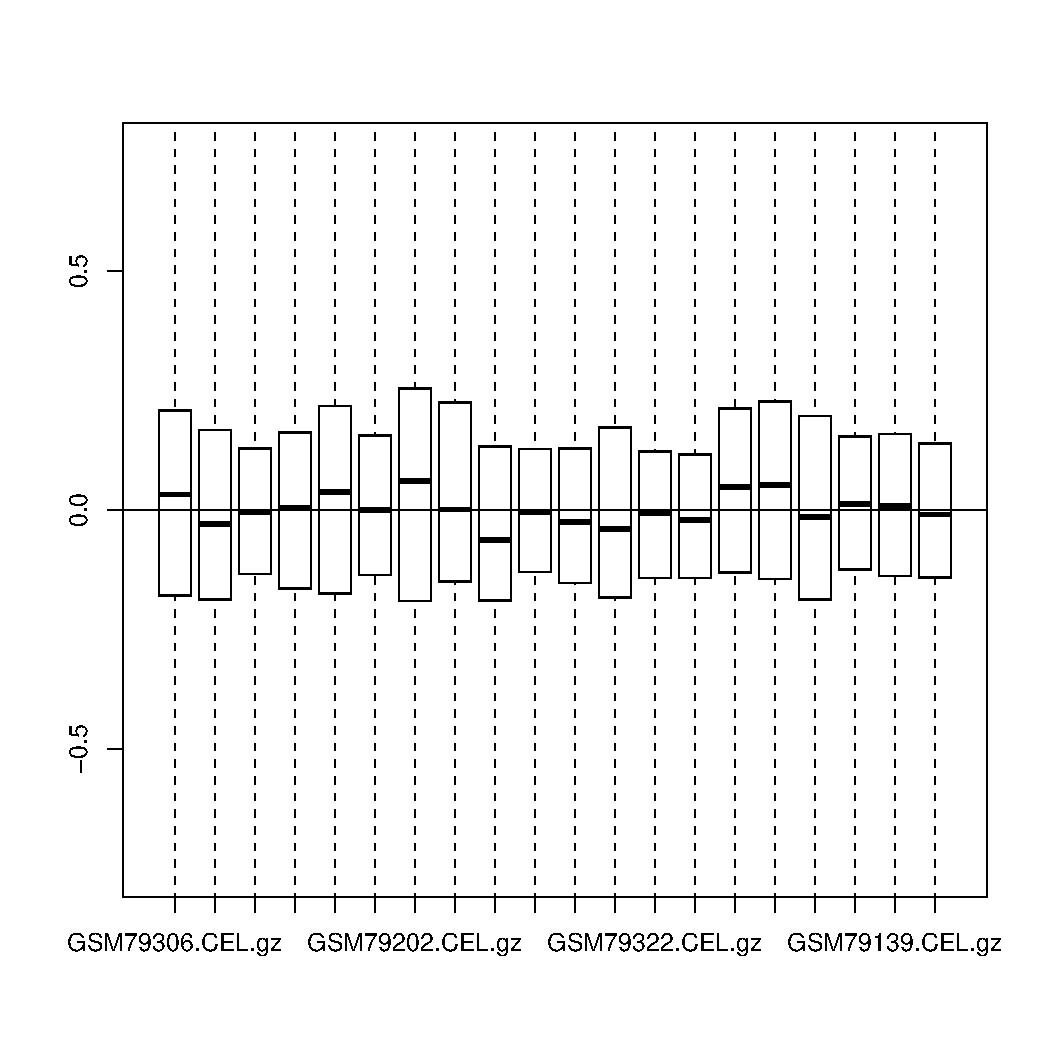
\includegraphics[width=0.45\textwidth]{A_RLEplot.pdf}}
\caption{$RLE$ plot for raw data of $A$ batch}
\label{fig:rleplot}
\end{figure}

\subsection{Preprocessing of Microarray Data. Background Correction and Normalization}
As no quality-control based filtering was needed, we proceeded to apply a background correction and normalize our data.We used the Robust Multi-chip Average Method (RMA) in order to correct and normalize, producing the $MA$ plot for already normalized data as a result (fig. ~\ref{fig:rmaplot}). The method discards the MM probes and considers that background noise and non-specific hybridization (B) and specific hybridization signal (S) are the two main components of the values from the PM probes. The new $MA$ plots show a significant decrease in the dispersion of the data after background correction and normalization.

\begin{figure}[h!]
\centerline{\fbox{\includegraphics[width=1\textwidth]{A_batch_RMA.png}}}
\caption{$MA$ plot for normalized data of $A$ batch}
\label{fig:rmaplot}
\end{figure}


\clearpage
\section{R Script}

\begin{verbatim}
# construct the AffyBatch object out of the extracted data
>library('affy')
>pData = read.table('phenodata_20.tab', row.names=1, header=TRUE,
+sep="\t")
>metadata = data.frame(labelDescription=c("p53 Status", "DLDA Classifier",
+"DLDA Error", "Elston histologic grade", "ER status", "PgR status",
+"Age at diagnosis", "Tumor Size (mm)", "Lymph Node Status",
+"DSS Time", "DSS Event"))
>phenoData = new("AnnotatedDataFrame", data=pData, varMetadata=metadata)
>file_content = read.table('gsm_A')
>A_files = as.character(file_content$V1)
>A_batch = ReadAffy(filenames = A_files, phenoData=phenoData)

# produce the MA plots for the raw data
>library(affyPLM)
>png('tex/A_MAplot.png', width=1920, height=1200)
>par(mfrow = c(4, 5))
>MAplot(A_batch)
>dev.off()

# produce the NUSE and RLE plots for the raw data
>pdf('tex/A_NUSEplot.pdf')
>NUSE(Pset)
>dev.off()
>pdf('tex/A_RLEplot.pdf')
>RLE(Pset)
>dev.off()

# calculate the values for the PM and MM probes
>apms <- pm(A_batch)
>amms <- mm(A_batch)

# produce the scatter plot
>pdf('tex/A_SCATTERplot.pdf')
>smoothScatter(log2(amms[, 1]), log2(apms[, 1]),
+xlab=expression(log[2] * "(MM) values"),
+ ylab=expression(log[2] * "(PM) values"), asp=1)
>dev.off()

# produce the plot of distribution of intensities
>pdf('tex/A_INTENSITY_DISTRIBplot.pdf')
>boxplot(A_batch, names=1:length(sampleNames(A_batch)),
+xlab="Chip A", ylab=expression(log[2] * "(intensity)"),
+main="Hybridization intensities distributions across
+20 subjects on the A chip")
>dev.off()

# use the RMA method: apply the background correction and normalize the data
>A_batch_RMA = rma(A_batch)

# produce the MA plots for the normalized data
>png('tex/A_batch_RMA.png', width=1920, height=1200)
>par(mfrow = c(4, 5))
>MAplot(A_batch_RMA)
>dev.off()
\end{verbatim}

\newpage
\section*{Appendix}
The randomly generated subset of GSE3494 dataset which was used for the analysis\\\\INDEX (ID)\\p53 seq mut status (p53+=mutant; p53-=wt)\\p53 DLDA classifier result (0=wt-like, 1=mt-like)\\DLDA error (1=yes, 0=no)\\Elston histologic grade\\ER status\\PgR status\\age at diagnosis\\tumor size (mm)\\Lymph node status\\DSS TIME (Disease-Specific Survival Time in years)\\DSS EVENT (Disease-Specific Survival EVENT; 1=death from breast cancer, 0=alive or censored )

\begin{center} \label{table}
\resizebox{14cm}{!} {
\begin{tabular}{||c|c|c|c|c|c|c|c|c|c|c|c|c||} \hline
patient ID & GSM & status & classifier & error & histologic grade & ER status & PGR status & age & tumor size (mm) & node status & DSS Time & DSS Event\\ \hline
X314B55 & 79306 & p53+ & 1 & 0 & G3 & ER- & PgR- & 38 & 30 & LN- & 9.583 & 1\\ \hline
X164B81 & 79165 & p53+ & 1 & 0 & G2 & ER- & PgR- & 62 & 23 & LN- & 11.333 & 0\\ \hline
X250C78 & 79253 & p53+ & 1 & 0 & G3 & ER- & PgR- & 75 & 18 & LN- & 2.667 & 0\\ \hline
X66A84 & 79340 & p53+ & 1 & 0 & G3 & ER+ & PgR- & 48 & 35 & LN+ & 1.417 & 1\\ \hline
X287C67 & 79287 & p53+ & 1 & 0 & G3 & ER+ & PgR+ & 37 & 20 & LN+ & 10 & 0\\ \hline
X189B83 & 79191	& p53+ & 1 & 0 & G2 & ER- & PgR- & 58 & 38 & LN- & NA & NA\\ \hline
X19C33	& 79202 & p53+ & 1 & 0 & G1 & ER+ & PgR+ & 61 & 31 & LN+ & 4.167 & 1 \\ \hline
X208C06	& 79211 & p53+ & 1 & 0 & G2 & ER+ & PgR+ & 67 & 22 & LN? & 0.083 & 0 \\ \hline
X50A91	& 79325 & p53+ & 0 & 1 & G2 & ER+ & PgR- & 47 & 22 & LN+ & 9.583 & 1 \\ \hline
X69A93	& 79342 & p53+ & 1 & 0 & G3 & ER+ & PgR+ & 62 & 50 & LN+ & 12.417 & 0\\ \hline
X231C80	& 79232 & p53- & 0 & 0 & G1 & ER+ & PgR+ & 56 & 22 & LN- & 10 & 1\\ \hline
X84A44	& 79354 & p53- & 0 & 0 & G2 & ER+ & PgR+ & 84 & 28 & LN- & 12.167 & 0\\ \hline
X47A87	& 79322 & p53- & 1 & 1 & G2 & ER- & PgR- & 61 & 53 & LN+ & 10.583 & 0\\ \hline
X152B99	& 79153 & p53- & 0 & 0 & G2 & ER+ & PgR+ & 83 & 18 & LN- & 2.083 & 0\\ \hline
X150B81	& 79161 & p53- & 0 & 0 & G2 & ER+ & PgR+ & 55 & 35 & LN+ & 11.417 & 0\\ \hline
X297C26	& 79296 & p53- & 0 & 0 & G2 & ER+ & PgR+ & 51 & 30 & LN+ & 9.917 & 0\\ \hline
X247C76	& 79249 & p53- & 0 & 0 & G2 & ER+ & PgR+ & 56 & 25 & LN- & 10.5 & 0\\ \hline
X48A46	& 79323 & p53- & 0 & 0 & G1 & ER+ & PgR+ & 78 & 38 & LN? & 1.833 & 0\\ \hline
X138B34	& 79139 & p53- & 0 & 0 & G1 & ER+ & PgR+ & 65 & 23 & LN+ & 11.5 & 0\\ \hline
X292C66	& 79293 & p53- & 0 & 0 & G2 & ER+ & PgR+ & 51 & 20 & LN- & 10 & 0\\ \hline\hline

\end{tabular}
}
\end{center}

\end{document}
